%!TEX root = Beschreibung_des_Vorhabens.tex

Figure nnn shows the principal components of the TraceSEC method. The pyramid symbolizes an extended quality model [26] REFanderes as described above. Since the selection, order, and details of those activities may differ between projects, TraceSEC will enable projects to map and configure respective parts of their development approach to the TraceSEC reference model. This is also used to accommodate various development styles.

Activities referring to a quality model (WP1) impose traces between quality model, other artifacts, and the activities (WP2). Raw traces gained from recording basic interactions must be reduced to a subset of security-relevant elements (WP3). They will be analyzed in depth (WP4) and prepared for value-adding steps (WP4). This interpretation and abstraction will require combining automated and a few manual steps. Resulting threads of traces, artifacts, and quality items will be used differently for development (WP6), problem handling (WP5), and continuous learning (WP7). Evaluation is an on-going process that runs in parallel (WP8).

\begin{figure} \centering
	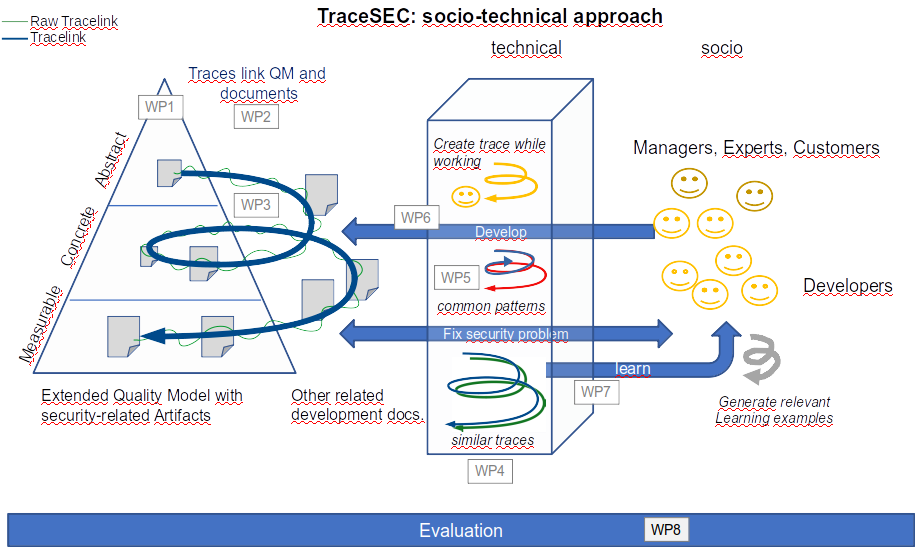
\includegraphics[width=1.0\textwidth]{resources/work-plan}
	\caption{Symolic representation of the TraceSEC-methods and its core components}
	\label{fig:work-plan}
\end{figure}

The work programme is organized around this structure. It starts by exploring and investigating what could and what should be added to an extended quality model for the three supported core activities (WP1). This will result in a reference model. It can be extended by trace links. Two issues are related: In WP2, we will identify and evaluate ways of collecting traces as a by-product. Whenever developers or stakeholders conduct a security-related activity, traces should be derived without extra effort. Given those raw traces, WP3 will develop and investigate techniques for assessing the relevance of trace elements. Trace candidates will be classified, interpreted, and abstracted to reusable units of knowledge (centered around a scenario). 

WP 4 will explore threads of traces and try to extract that is meaningful to the stakeholders. In WPs 5-7, the above-mentioned three core activities will be investigated with respect to the quality models, traces, and scenarios that can be derived from them. WP5 is an ordinary development step which may or may not have relevance for security. We use heuristics and automated classifiers, which may require additional human intervention to come to a conclusion. WP6 represents the detailed diagnosis and analysis of a current security problem. Both WP5 and WP6 build on identification of patterns and similarities of scenarios (documents and threads). Information can be extracted from several similar traces. Workplace learning is supported by contextualized examples and exercises from the same source; they will be generated from the same web of traces and scenarios. Since they stem from that same company context, they are implicitly highly relevant for this context. WP 7 will generate valuable educational material from threads for developers in their development context.

\begin{tabular}{|p{6cm}|p{10cm}|}
	\hline 
	\textbf{Work package} & \textbf{Deliverable} \\ 
	\hline 
	WP1: Security-Related Contents of a fine-grained QM & 1-Report/publication: What can be included, potential benefit, evaluation results.\\
	2-Reference model. \\ 
	\hline 
	WP2: Creation of Trace-Links as a By-Product of Activities & List of useful content items and how they can be captured as by-product (report) \\ 
	\hline 
	WP3: Interpretation of Trace-Links (relevance, abstraction, classification) & Report and associated demonstration software: Techniques and mechanisms for interpreting raw trace links (software demonstrators, process for semi-automated parts) \\ 
	\hline 
	WP4: In-Depth Analysis of Artifacts, facilitated by QM and trace links & Report and associated demonstration software: Techniques and mechanisms for analysis \\ 
	\hline 
	WP5: What led to this error? Trace-based forensics &  \\ 
	\hline 
	WP6: Suggestion of security mechanisms and processes &  \\ 
	\hline 
	WP7: Contextualized learning & Algorithms and demonstrators for extracting relevant parts from traces/threads, and for transforming them to learning units (e.g. videos) \\ 
	\hline 
	WP8: Evaluation on Realistic Use Cases & Report on developer support and experience \\ 
	\hline 
\end{tabular} 

\paragraph*{WP1: Security-Related Contents of a Fine-Grained Quality Model}
Using a quality model as fundamental artifact is a key decision in TraceSEC. The purpose of a quality model usually is to represent those non-functional requirements [7] that can be assigned to quality attributes that are important for a given project. Depending on the size of the project and on the significance of those quality aspects, the selection will be made by or together with customer representatives. There are formal and informal representations, automated and semi-automated techniques. In the case of market-driven development [13], the development organization has to decide, for example, on the relative importance of security vs. ease of use (see Running Example). 

As described above, not all projects refine quality models beyond this first layer of prioritization. In TraceSEC, we rely on a second layer of concrete components or use cases or situations and threats in which security is essential and where security requirements can be understood in more detail. This is the basis of a third layer of indicators and metrics (measurement) of those particular sub-aspects of security. On all layers, there may be other quality aspects, refinements, and metrics, too. If they are related or in contrast with security, we also want to represent this in our extended quality model. However, other quality aspects will only be represented where they relate to security, too. In contrast to most projects, our reference model for quality (including security) will be extended to include or reference (in separate artifacts) all heuristics, rationale, and mechanisms related to security. 

It is the purpose of WP1 to collect elements and aspects of security, reaching from requirements and priorities to vulnerable code patterns and heuristics for monitoring. There are two basic activities in WP1: (1) gathering candidates and (2) evaluating their relevance and significance. While (1) will be supported by our own experience from previous projects, an update of earlier literature reviews \todo[inline]{REFhabenWirEine?} and input from companies, (2) will identify irrelevant candidates and candidates that are doublets or will not advance research (exclusion criterion). The principal inclusion criterion for relevance will be whether we can find a use case or misuse case that references this kind of element. We do not seek completeness, but rather want to cover a broad range of definitely useful elements. This choice will lead to a rich selection of elements, but limit effort to a feasible level for a basic research project. 

This reference model with rationale and application examples will be the basic building material for projects. They will instantiate the elements, which will be a socio-technical activity: human decisions on informal levels will be included as much as technical monitoring and formal analysis.

Since all adopted elements in this rich quality model must be justified by their occurrence in a relevant product development, it will be possible to map them back to real projects. At this point, we do not distinguish by project characteristics or type, as long as the relevance is substantiated. 

The research questions in WP1 are:
\begin{description}
	\item[RQ1.1] What are relevant elements associated with security, and how can they be organized within extended quality models?
	\item[RQ1.2] How can information be organized in quality models to be usable for both humans and machines?
\end{description}

Deliverable:  
\begin{description}
\item[D1.1] Reference model and catalogue of elements.
\end{description}

The result of WP1 is a reference model with relevant elements identified, and a link or reference or example to the witnessing application in which it showed its relevance. Resulting instantiations (quality models) will be the source and reference for security knowledge in all three core activities. These knowledge elements will be connected by trace links (WP2, 3).


\paragraph*{WP2: Creation of Trace-Links as a By-Product of Development Activities}
In WP1, we collect and analyze security-related elements in a software project. Their relevance is supported by examples, but we do not investigate in WP1 how those elements are created or how they depend on each other in detail. WP2, in contrast, will identify sources and techniques to elicit security-related traces on all levels This work package builds on related work for generating trace links or candidate links REF++advancing. It will specialize those generic approaches, such as the requirements traceability matrix RTM, towards security activities and benefits for security. This challenge will be addressed with a spectrum of socio-technical approaches. In the early or visionary phases of a project, there will be more informal considerations.

In traditional processes or agile processes, different kinds of artifacts are created and different kinds of tools are used. Different traces can be elicited, and they come in a different order. In this work package we investigate how these differences affect the elicitation as a by-product and how the traces can be made available for the following interpretation and analysis. As outlined above, we intend to reduce the effort by generating traces as a by-product. In addition, we will raise the benefit by using and reusing traces and connected information for all three core activities (development, problem solving, learning).

Example: They may lead, e.g., to top-layer decisions in the Running Example to prioritize security higher after the incident with the router. While the decision by itself may reside on the top layer of the quality model (“security is high priority. Rationale: Leaks may threaten personal medical data (GDPR)”), we will try to trace this decision from its triggers (the incident and a press release) over considered options (see Example) to the final resolution (“prioritize higher”) and its consequences.

Identification will include a variety of sources. The goal of WP2 is to include at least one instance of each type:
\begin{enumerate}
\item Explicit traditional traces from tools like Doors REF. They constitute the current state of practice in advanced projects. Less advanced projects often neglect traces at all.
\item  Automated repository mining: Patterns of reading-activity-writing indicate an information flow from the read to the written elements. 
\item  Negotiations among stakeholders about relative importance of quality aspects (e.g., usability vs. security) must be captured in a different way. We have experience in constructing tailor-made and privacy-respecting observation apps REF. They may, for example, require basic manual entries that are anonymized and pre-evaluated before they are ever stored.
\item  Interactions of developers during security-related development activities could be monitored technically or semi-automated, as sketched in (c).
\item  When developers interact with tools (e.g., CogniCrypt for generating secure code or nnnOtherTool), capturing a detailed trace automatically should be easier, but must be weighed with personal and privacy concerns.
\item  Run-time monitoring is yet another source of fine-grained traces. Again, not everything that can technically be collected should be included. It will be one of the questions in WP2 to investigate potentials and balance with effort and competing concerns.
\item  We will use established mining techniques REF and integrate informal traces from (a) and (c) using the information flow visualization technique FLOW [29] [31] to gain an overview and a socio-technical model of what is being elicited.
\end{enumerate}

It is important not only to elicit implausible or meaningless traces, but also to keep the number of traces as low as possible, to avoid the risk of bad maintenance or bad performance of any technical processing of traces.

Research Questions:
\begin{description}
\item[RQ2.1]  What are (existing or new) mechanisms for capturing traces that can be used to connect the security elements identified in WP1
\item[RQ2.2] How can raw traces be cleaned and filtered to achieve plausible and meaningful traces only?
\item[RQ2.3] How do different types of development processes affect the creation of trace links?
\end{description}

Deliverables: 
\begin{description}
\item[D2.1] A catalogue of elicitation techniques and related types of traces that are security-related and touch on elements of the extended quality models (WP1). 
\item[D2.2] Techniques (description and software demonstrators) for filtering out useless and implausible traces or parts of traces.
\end{description}

The result of WP2 is a catalogue of all identified elicitation techniques and techniques for filtering traces They can be used to build up a model of relevant “raw” traces, with connections to the QM, ready to be interpreted and analyzed in WP3 and 4.

\paragraph*{WP3: Interpretation of Trace Links for Adding Value}
In WP1, elements (models, decision, algorithms and heuristics) are identified. They are connected in the context of original use through traces extracted in WP2. Both WP1 and WP2 focus on finding opportunities and filtering out implausible and overly voluminous elements and traces. The resulting set can now be prepared for reuse and value-added exchange between the three core activities (development, problem analysis, learning). 

We will explore operations on traces that connect quality model elements and artifacts. We call these constructs “threads”. These operations are specific for the intended use in TraceSEC, but not limited to a single use within TraceSEC. The value of threads and traces will be weighed against the effort to create them. Observing activities and generating traces will reduce effort, while mechanisms for comparing and reusing them will add value REFvalueB.

Examples include:
\begin{itemize}
\item Apply semantic filtering of traces. Longer sequences that do not touch on security elements can be hidden or removed. This helps to abstract to a higher level and reach a better overview. 
\item Soft matching of threads. If there are sub-sequences of common or similar security activities and elements in different traces, it may be interesting to look at the rest. For example, if a project starts with the same unusual repetition of decisions as a previous one, it could be interesting to see how that earlier project continued.
\end{itemize}

All operations can be used in at least one of the specific areas covered by WP6 (development), WP5 (problem analysis), and WP7 (learning). In most cases, they assist in preparing and reusing knowledge across these three core activities of TraceSEC. WP3 turns raw threads in meaningful ones.

Research Questions
\begin{description}
	\item[RQ3.1]	What are effective techniques to carry out operations on threads, as exemplified above?
	\item[RQ3.2]	How do machine learning techniques perform for this specific purpose, compared to socio-technical techniques that combine automated matching with human involvement?
\end{description}

Deliverable
\begin{description}
	\item[D3] Report on algorithms and mechanisms investigated, with study design and empirical results for comparison. 
\end{description}

The resulting report of WP3 covers both research questions, since RQ3.2 refines RQ3.1. 

\paragraph*{WP4: In-Depth Analysis of Artifacts, Facilitated by QM and Trace Links}
WP4 continues the semantic analysis. While WP1 and WP2 have removed implausible elements, WP3 entered the level of semantics, by investigating thread-specific operations that can be used for several purposes. WP4 goes beyond generic operations and explores options for analysis that is meaningful for project participants.

\textbf{Higher-level semantic interpretations of a thread} include:

\subparagraph*{Does a given thread from development comply to a given development process?} This question will use a simplified set of indicators for compliance. For example, Zazworka et al. [37] checked a development repository and analyzed whether there were always tests committed before source code. This was interpreted as a compliance criterion for test first. It is important to note that there is a trade-off between simple criteria and reliable results. In this example, Zazworka et al. did not check which tests referred to what part of code. Simplification was prioritized over reliability; in other words, only clear violations were to be reported (e.g., if there was no test at all before coding started).

\subparagraph*{Is this sequence of reading and writing artifacts or security elements typical?} In this type of question, there is no predefined process. The growing set of threads constitutes what is considered “typical”. We will apply machine learning for the statistical part of the analysis. Following our socio-technical approach, human interventions may be considered, too.

\subparagraph{Is a quality model populated in an unexpected way?} Patterns can be searched on threads (above) but also on elements of the quality model. For example, a quality model with lower-layer elements only (monitors, but no prioritization or concrete examples) may be too technology-focused, missing strategic awareness. This can in turn indicate a risk of ignoring other vulnerabilities, due to tunnel vision.

There are many hypotheses and experiences that can \textbf{evaluate a situation formalized on sets of threats}: Can we interpret repetition in a thread as problem fixing, or revision of a decision? This type of questions will probably lead to heuristics. 

Research Questions
\begin{description}
	\item[RQ4.1]	Is it feasible to recognize higher-level semantic similarities and potential problems by comparing and merging threads?
	\item[RQ4.2]	How can information captured in the quality models be utilized to provide more sophisticated low-level security checks?
\end{description}
	
Deliverable
\begin{description}
	\item[D4]	Scientific report (publication) on the Research Question. Feasibility would be demonstrated with at least two examples.
\end{description}

\paragraph*{WP5: What Led to This Error? Trace-based Forensics}
Security problems often have several causes that must come together. In the Running Example, nnn.
It is particularly difficult to reconstruct and diagnose the root causes of an attack or a privacy problem. An important precondition is a good record of potentially relevant events and decisions. Fine-grained tracing can be helpful. While it is difficult to remember details, and join them with details of another cause, threads may help – in particular since they are not limited to threads within a repository or on a computer. We envision socio-technical threads on all aspects of security.

Using the types of elements (WP1), traces (WP2), plausible (W3) and pre-interpreted threads (WP4) mentioned above, WP5 addresses one of the core activities related to security: Diagnosis and analysis of problems, which could be called trace-based forensics.

WP4 has two parts (leaving a trace and using a trace):
\begin{itemize}
\item Whenever forensic analysis of a real problem occurs, security experts search the (extended!) knowledge-base for symptoms and causes. This activity is human-driven and exploits the rare resource of security experts. Their experience enables them to identify suspicious parts faster. As they do that, they leave a trace. 
\item Earlier traces can be used to inspire less-experienced developers in problem analysis. Using soft matching from WP3 and WP4, they can reuse similar threads to look at the right places.
\item Following the model of FOCUS [21] [34], a new search can again create a trace. After the first steps, it is only a partial trace. Nevertheless, soft-matching the prefix against successful solution threads can help to identify promising threads to continue with. 
\item Perfect matches and a ready-made solution based on old cases will be the exception rather than the rule. However, much can be done on the side if most tracing and soft-matching does not require human effort (by-product [24]). That leaves human capacity for closing the gap between reused knowledge (threads) and actual problem context (thread again).
\item Entire sets of forensics can be collected. They represent typical cases and implicitly represent how frequently they occur in this environment. 
\end{itemize}

Research Question
\begin{description}
	\item[RQ5]	How effective are threads as knowledge representation for future problem analysis?
\end{description}
	
Deliverable
\begin{description}
	\item[D5] Report on effectiveness, potential, identified limits of thread-based problem analysis
\end{description}

\paragraph*{WP6: Suggestion of Security Mechanisms and Processes}
\begin{itemize}
\item Klare Empfehlung aus den alten QMen (anonymisiert), was sich bewährt hat
\item Code generieren
\item Heuristcs für Monitoring und Laufzeitfehler
\item Kriterien-Beispiele, um etwas zu beurteilen
\item Fälle aus anderen (anonymisierten) Artifacts, Testfällen usw., wie man weiterarbeiten kann.
\item Resultat:  Recommendations for current development
\end{itemize}

\paragraph*{WP7: Contextualized Learning}
There is a growing number of security lectures at Universities. Novice developers have a better likelihood to be aware of security. However, they are still a minority, and even that minority needs to keep learning, as attack knowledge grows and poses new security challenges. Learning on security is a continuous necessity, and it should consist of individual and organizational contributions to be effective.

WP7 will pick up general operations from WP3 and higher-level matching and interpretation from other work packages. Based on all these materials and thread-based knowledge representation, TraceSEC enables concrete and contextualized learning, closing the loop from development over problem analysis, to workplace learning on demand.

Learning on demand [6] occurs only when there is an actual demand, such as a security problem identified at run-time. Upon this trigger, the problem must be identified and solved. WP5 addresses this core activity. However, others can benefit from that solution.

WP7 has the vision to use appropriate threads (e.g., showing a problem and the process to solve it). They should be simplified (using mechanisms as developed in WP3 and WP4) and transferred to a representation that is better suited for learning. NnnREF presents guidelines for creating video tutorials. In [14], Karras and Schneider report on quality requirements and guidelines for creating “good-enough video” in software engineering. For WP7, it will be essential to strip threads of ballast and to re-construct a story. If there are multi-media elements in the quality model (WP1), they can be used; fine-grained technical traces from the repository may not include screen casts. But they can easily be generated or re-created following a detailed trace. FOCUS exemplifies a strategy to capture video as a by-product of demonstrating a prototype. 

WP7 will collect requirements for getting valuable educational material as by-product. We expect to implement some of those requirements in a socio-technical demonstrator, again combining the strengths of computers and humans. Additional information should be captured in a light-weight way, such as the cost and consequences of an error, external events.

As usual for organizational learning, individual learning is a crucial ingredient [26]. To lift it to an organizational level, some of the knowledge must be externalized [17] and stored in a repository for other members of the organization. In TraceSEC, the collection of threads constitutes the representation to store knowledge. More than simply storing it, the above-mentioned work packages investigate thread-based opportunities to benefit from core activities of others, and from sophisticated socio-technical support developed in TraceSEC.

Research Questions
\begin{description}
	\item[RQ7.1]	Do threads contain sufficient material to construct educational examples (maybe manually)?
	\item[RQ7.2]	How could existing parts be collected and transferred automatically, indicating what remains to be done by humans?
	\item[RQ7.3]	How can user decisions and changing public knowledge be automatically reflected in future automatically executed analyses.
\end{description}

Deliverables
\begin{description}
	\item[D7] Case study showing the feasibility of transfer. Maybe semi-automated. 
\end{description}

\paragraph*{WP8: Evaluation on Realistic Use Cases}
Our approach includes technical artifacts that can be continuously improved over time, and it also includes humans with different levels of experience who learn during the application of our approach. Therefore, an exactly repeatable case study is not achievable. To evaluate the overall approach regarding the project objectives, we will conduct user studies with realistic use cases, based on our experience with industry partners \todo[inline]{hier eine bessere Formulierung finden}.

The user studies will include developers with different levels of experience that use our approach and tool prototype in a set up development environment for a given set of tasks. Their activities and the recommendations and activities of the software will be logged as well as the intentions of the users using the thinking aloud technique \cite{thinkingAloud}. A control group will execute the same tasks without the approach. We expect the results of the treatment group to be better than the control group, because they have additional support. Interesting is the degree of developer support, measured in the number of successfully finished tasks and the time required, and the subjective experience of the developers in both groups using the thinking aloud protocol.

Research Questions
\begin{description}
	\item[RQ8.1]	Does the approach increase developer efficiency and effectiveness, and to which degree?
	\item[RQ8.2]	What are the experiences and thoughts of developers using the approach, compared to developers that do not use the approach?
\end{description}

Deliverables
\begin{description}
	\item[D8] Report on the evaluation
\end{description}

\paragraph*{Plan and Effort}
As outlined in Sec. nnn, the applicants approach the topic of TraceSEC from different angles: Jan Jürjens and his team has a long record of security modeling (e.g., in UMLsec [12]) and formal techniques to verify REF and ensure security REF. Kurt Schneider and his group focus on socio-technical aspects of software engineering, such as elicitation and validation of requirements and explainability [5]. They build tools to support the collaboration of technology and humans in a software engineering context (e.g., FOCUS [21], AppForMeetings, HeRA [11]). Their successful cooperation in SecVolution (SPP 1593) showed their ability to create solutions together that none of them could create on their own. 

As a consequence, work package leads are assigned to those focusing on a particular topic; however, both groups address their particular perspective in all work packages and will collaborate throughout all parts of the project. Therefore, the differences in planned person months is different between the groups, but not very different. The socio-technical approach requires constant exchange of ideas and results. Table nnn provides an overview of the effort devoted to the work packages by the two applicant groups. 

Table nnn:
\todo[inline]{Hier ein Vorschlag, in den WP 8 miteingerechnet ist und der etwas mehr Profil zeigt}

\todo[inline]{Hier die Tabelle mit den WP und PM}

Fig. nnn shows the distribution of effort in the planned work packages over time. Work progresses along work packages WP1-WP7. It is complemented by the cross-cutting evaluation work package WP8. Since both groups from Koblenz and Hannover work on different aspects of each work package, there is less need for parallel work packages. Of course, insights from a work package may lead to refine earlier work package results. This limited revision effort is planned in the latter work packages.

\todo[inline]{Hier ein Projektplan}
